\chapter{Desenvolvimento}
\label{chap:desen_test}
\begin{flushright}
	"Insanidade é continuar fazendo sempre as mesmas coisas, \\ 
	esperando resultados diferentes." \\
	\ \\
	(Albert Einstein)
\end{flushright}

Para obter de forma efetiva o proposto na metodologia, foram elaborados dois conjuntos principais de entregáveis: os Tutoriais, e o Kit Físico. Após finalização do projeto, os Tutoriais se encontram em domínio virtual, na Wiki do repositório da Learnbotics no Github, e o Kit Físico foi fabricado e montado. A seguir encontra-se uma melhor explicação de como esses resultados foram obtidos.

\section{Preparação do Robô}
Para que tudo o que foi pensado pelo projeto pudesse ser desenvolvido e passado ao usuário, uma escolha cuidadosa do hardware foi efetuada. Posteriormente, uma configuração e testes deste hardware foram também realizados.

\subsection{Hardware}

\subsubsection{Testes de Hardware}
<<<<<<< HEAD
Como apresentado anteriormente, o kit físico irá conter os seguintes componentes:
\begin{table}
	\centering
	\begin{small}
		\caption{Componentes constituintes do kit fisíco.} \label{Tabela1}
		\begin{tabular}{cc}
			\hline
			Componentes              & Quantidade\\
			\hline
			Raspberry Pi3B              & 1 \\
			Dynamixel MX-28			    & 2 \\
			Câmera RGB		            & 1 \\
			Rodas emborrachadas		    & 2 \\
			Roda boba		            & 1 \\
			Cabos e conexões            & x \\
			Bateria 			        & 1 \\
			\hline
		\end{tabular}
	\end{small}
\end{table}

Muito dos componentes acima são comumente utilizados, tendo uma alta qualidade atrelada, porém, somente quando atreladas à um uso comum. Como o projeto deste trabalho envolvia o uso de uma raspberry, tornou-se necessário o teste de integração entre os componentes e a raspberry.
\subsubsection{Sistema operacional da Raspberry}

Para a utilização dos ROS e OpenCV é preferível que estes estejam instalados em um SO (Sistema Operacional) com base em LINUX e com suporte ao ROS e OpenCV. Inicialmente foi testado o Ubuntu 16.04 server. Este SO é um derivativo do Ubuntu 16.04, a única diferença é que este não compõe a parte gráfica. Teoricamente, o Ubuntu server seria o Sistema operacional perfeito para a aplicação deste trabalho, por ser um sistema sólido, amplamente testado e que tem um dos melhores suportes às ferramentas utilizadas. Com tudo, há um pequeno problema na utilização dele, que não há suporte gráfico, ou seja, o aluno de cara teria um grande estranhamento de apenas utilizar o terminal para conseguir fazer as aplicações e desafios compostos no kit. 

Com isso, foi preferível instalar o SO Raspbian, uma derivação do Debian. O Raspbian é um sistema operacional otimizado e próprio para a Raspberry, tendo suporte para ROS e OpenCV. Não é possível instalar o SO Ubuntu 16.04 com gráficos pois, a Raspberry não consegue comportar ele, já que ela conta com uma memória gráfica limitada.

O que é interessante neste SO que ele é disponibilizado pela própria Raspberry e mantido por ela. Com isso, este sistema vem com diversas aplicações educacionais, e possíveis projetos que se o aluno quiser explorar, poderá encontrar infinitas finalidades.

Para instalação do SO na Raspberry, foram utilizados os seguintes materiais, mostrados na figura \ref{fig:SO}:

\begin{enumerate}
	\item Raspberry PI 3B+
	\item Cartão SD 32 GB
	\item Imagem do Sistema Operacional

\end{enumerate}

\begin{figure}[H]
	\centering
	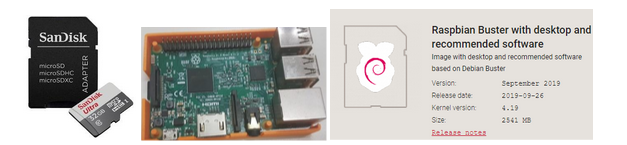
\includegraphics[scale=0.8, angle=0]{Figures/so.png}
	\caption{Componentes necessários para instalar o SO}
	\label{fig:SO}
\end{figure}

A instalação do SO em si foi seguindo o tutorial disposto no próprio site da \cite{RASPB}, o raspberrypi.org. Lá contém tudo que é necessário para instalar, os passos a serem seguidos e como otimizar a Raspberry.
\subsubsection{ROS na Raspberry}
Para o comprimento dos requisitos funcionais do kit, faz-se necessário a instalação do framework de robótica ROS. Este passo normalmente é fácil e intuitivo, porém, quando se trata de uma ARM (Advanced RISC Machine) a instalação de frameworks como este tornam-se mais complexo. Esta dificuldade é consequência por dois fatores:

\begin{enumerate}
	\item A arquitetura é mais simples se comparado com processadores utilizados em computadores pessoais;
	\item O Sistema Operacional (SO) utilizado é o Raspbian, um SO baseado em Linux próprio para a Raspberry. 
\end{enumerate}

Por conta destes dois fatores, a instalação do framework não pode ser feita da mesma forma que é em um computador normal. Felizmente, há diversos tutoriais disponíveis na Internet para o auxílio desta tarefa, porém, isso não fez diminuir o nível esforço para o comprimento dela. 

Tendo em vista esta complexidade, a equipe repensou como iria entregar o kit, mudando assim o requisito que o aluno deveria instalar o ROS na Raspberry. O que é interessante analisar é que o intuito deste trabalho é apresentar de forma fácil e prática o mundo da robótica aplicada para os alunos, então, para que não houvessem desistências prematuras do curso, foi preferido entregar o ROS já incluso.
\subsubsection{Instalação do ROS na Raspberry}

Inicialmente, foi utilizado o SO Ubuntu 16.04 server. Neste sistema a instalação do framework ROS foi simples, já que este sistema é amplamente utilizado pela comunidade, sendo assim, tem uma maior suporte.

Para ele, foi feito uma conexão via SSH, utilizando as entradas TX-RX da raspberry. Este tipo de conexão facilita a instalação, já que, pela raspberry somente havia o terminal, já que não havia a parte gráfica. A imagem \ref{fig:txrx} abaixo, mostra os componentes utilizados para a instalação.

\begin{figure}[H]
	\centering
	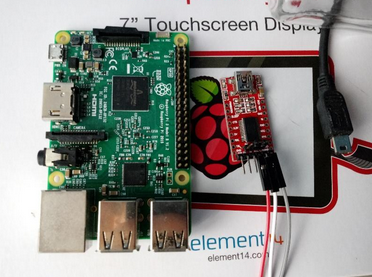
\includegraphics[scale=0.8, angle=0]{Figures/TX-RXconexao.png}
	\caption{Componentes necessários para instalar o ROS}
	\label{fig:txrx}
\end{figure}

Como previamente comentado, foi feito a mudança do Ubuntu para o Raspbian. Com isso, não se fez necessário a conexão por via TX-RX, já que neste caso, havia o componente gráfico no SO.

Para a instalação do ROS no Rasbpian, foi seguido o tutorial disponível no próprio site do ROS, o ROS.org. Porém, houveram alguns problemas com a instalação do Framework neste SO, desde problemas com dependências, com o próprio ROS etc. Estes percalços ocasionaram em um atraso de alguns dias no projeto, já que até então, não eram conhecidos e mapeados. 

\subsubsection{Instalação do OPENCV na Raspberry}
Para as aplicações de visão computacional, deve-se utilizar o OpenCV. Este contém inúmeras bibliotecas que viabilizam e possibilitam a identificação de cores, marcos fiduciais etc. Com isso, faz-se necessário a instalação desta ferramenta na Raspberry a fim de possibilitar ao aluno trabalhar com os princípios da visão computacional.

Há inúmeros tutoriais dispostos na internet para a instalação do OpenCV no sistema da Raspberry, especialmente com o Raspbian. Porém, a complexidade é tão alta quanto a instalação do ROS, por isso, a equipe concluiu que tanto o ROS quanto o OpenCV iriam ser entregues instalados na Raspberry.

Para testar se o OpenCV foi instalado corretamente, foi testado um algoritmo simples de identificação de Arucos, o resultado pode ser visto na figura \ref{fig:aruco1} logo abaixo. Este mesmo algoritmo está disposto na WIKI no Github do \cite{wikilearn}.

\begin{figure}[H]
	\centering
	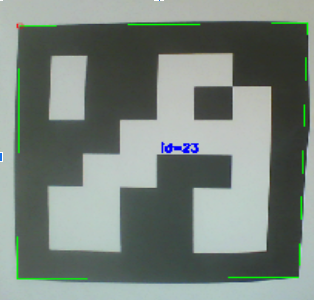
\includegraphics[scale=0.8, angle=0]{Figures/aruco1.png}
	\caption{Aruco de teste}
	\label{fig:aruco1}
\end{figure}

\subsection{Software}

=======

\subsection{Software}

>>>>>>> desenv
\subsubsection{Testes de Software}

\section{Tutoriais}
De forma a melhor organizar a elaboração do conteúdo dos tutoriais, uma divisão dos mesmos foi feita de acordo com o assunto abordado, ocasionando assim uma menor abrangência de assuntos a serem pesquisados, de conteúdos a serem concentrados e de novas interpretações a serem elaboradas. As subseções a seguir tratarão de partes específicas dos tutoriais.

\subsection{Um Breve Histórico da Robótica}
siaufgasiogfçwaugfsçfçsuaigfawgfçksgfiauçgwfgsfsaf fsiuafawfioashf saif sfiaywo fasfhaufaw fsifshaf wif saif w

\subsection{Introdução à Robótica atual e Alguns Conceitos Básicos}

\subsection{Introdução à Atuação}
Para que o estudante possa compreender de uma forma mais aprofundada o que está fazendo, antes de começar a mexer com os Dynamixels, uma pequena introdução a atuação foi elaborada.

Essa Introdução trata de uma forma simplificada do conceito de atuadores, de tipos de atuadores, de conversão de energia, e apresenta exemplos cotidianos de atuadores explicando seu funcionamento e aprofundando um pouco mais os conceitos de conversão de energia. \cite{tutAtua}

\subsection{Introdução à Visão Computacional}
Para o ensino de visão computacional apresentado na wiki do Github do Learnbotics \cite{wikilearn}, foi-se pensado na explanação dos conceitos de forma branda e intuitiva, já que, conceitos que se relacionam com visão computacional podem torna-se um tanto rebuscados quando buscados na bibliografia. Os principais conceitos abordados foram:
\begin{itemize}
	\item O uso da visão computacional;
	\item Características  (\textit{Features})
	\item Cantos, arestas e linhas (\textit{Corners,edges e lines})
	\item OpenCV
	\item Segmentação e identificação de cores
	\item Marcos fiduciais
	\item Pose
	\item Identificação de arucos
	
\end{itemize}

Os conceitos apresentados são suficientes para o objetivo do trabalho. Após a construção destes textos na wiki \cite{tutVis}, a equipe disponibilizou para uma pequena amostragem de pessoas a fim de receber feedbacks. Dentro desta amostra, haviam pessoas que trabalhavam com o assunto, que conheciam o uso e que não havia conhecimento prévio de visão computacional. Os principais tópicos abordados nos feedbacks foram:

\begin{itemize}
	\item Boa didática;
	\item Maior número de exemplos nos conteúdos abordados
	\item Conceitos apresentados de forma correta e correlacionando com exemplos do cotidiano
	\item Pequenos erros de digitação e ortografia
\end{itemize}

Os feedbacks, em resumo, foram positivos dos três grupos, tendo como consequência o auxílio a equipe a alcançar de forma satisfatória o intuito de explanar satisfatoriamente a área da visão computacional.

Como previamente abordado neste trabalho, um dos métodos de ensino proposto pela equipe foi a apresentação de desafios. Nos tutoriais foram apresentados os conceitos atrelados à desafios. Estes desafios tinham como intuito a validação dos temas abordados. Um exemplo de desafio proposto, foi o de segmentação de cores, no qual o usuário deve segmentar a cor azul. Para que o aluno conseguisse ter êxito neste desafio, a equipe apresentou  um algoritmo de segmentação da cor vermelha, previamente testado. O resultado pode ser observado na figura \ref{fig:vermelho} abaixo:

\begin{figure}[H]
	\centering
	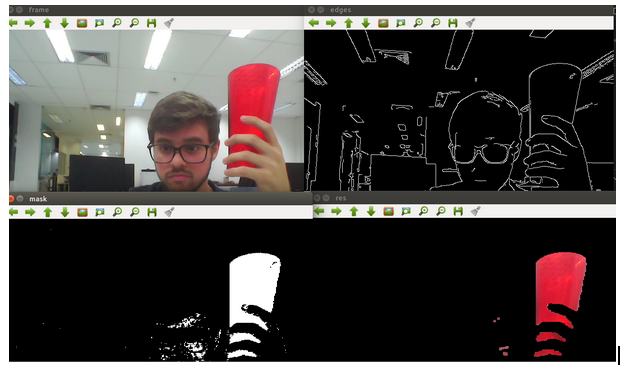
\includegraphics[scale=0.75, angle=0]{Figures/vermelho.png}
	\caption{Exemplo de segmentação de cores}
	\label{fig:vermelho}
\end{figure}
\subsection{Tutoriais da Raspberry Pi}

\subsection{Tutoriais dos Dynamixels}
Após ter tido contato com o conceito de atuadores, o estudante irá encontrar também um tutorial que faz uma introdução aos servo-motores inteligentes Dynamixel$^{TM}$.

Neste tutorial são apresentados os servo-motores inteligentes, suas diferenças para servo-motores comuns, suas vantagens sobre os comuns, qual o papel destes servo-motores no robô e no kit físico e mais precisamente porquê escolhemos utilizar os Dynamixels, e não servo-motores comuns. \cite{tutDyna}


\subsection{Tutoriais do ROS}
Tendo em vista a ídeia de apresentar ao estudante ferramentas que são de fato utilizadas por profissionais da área, buscamos realizar um material completo sobre as partes iniciais de utilização do framework ROS.

Devido ao nível de conteúdo que é abordado nos tutoriais nativos do ROS, foi feita uma análise de relevância dos conteúdos e uma reescrita completa do conteúdo abordado, trazendo novas abordagens para passar esse conhecimento para o estudante.

Este tutorial foi dividido em quatro partes, sendo elas, em ordem:
\begin{itemize}
	\item Introdução: O que é o ROS e como funciona;
	\item Conceitos Básicos: Apresentação de terminologia e conceitos base utilizados pela comunidade do ROS.
	\item Entendendo como Funciona o ROS: Apresentação de conteúdo novo que foi elaborado com base em analogias para facilitar o entendimento do estudante sobre a ferramenta.
	\item Tutoriais do ROS: Os Tutoriais de fato, onde o aluno irá aprender a configurar e utilizar o ROS.
\end{itemize}

A parte quatro, ou parte dos tutoriais de fato, aborda todos os conceitos de nível iniciante apresentados nos tutoriais oficiais do ROS. Porém estes conceitos foram demonstrados de forma mais simplificada, com linguagem mais simples e de forma acompanhada passo a passo para uma melhor assimilação do estudante.

Todos os tutoriais foram traduzidos do inglês para o poruguês, visando assim facilitar o acesso à uma amostragem maior de estudantes. \cite{tutROS}

\subsection{Apresentação dos Scripts de Cinemática}
Nesta parte dos tutoriais o estudante terá acesso ao programa que fará com que o seu robô ande. Além disso será ensinado também como o estudante deve proceder para que transforme seu código em um código executável e para rodá-lo.

De forma a estimular o estudante, uma análise mais minusciosa do código, com comentários parte a parte também foi feita. A partir da explicação do que os comandos do programa fazem o estudante terá condições de alterá-lo para concluir etapas e descobrir coisas por si só.

Para finalizar, o tutorial apresenta um desafio para que o estudante de fato assimile o que lhe está sendo proposto, alterando o código e vendo na prática o que isso ocasiona. \cite{tutCinemat}
<<<<<<< HEAD


=======
>>>>>>> desenv

\subsection{Integração dos assuntos anteriores}
Como validação de todos os conceitos apresentados na wiki do github \cite{wikiLearn}, a equipe pensou em um desafio que aliasse a visão computacional com os conceitos abordados de cinemática para um robô diferencial. 

Inicialmente foi pensado um robô seguidor de cores, porém, este não iria abranger alguns conceitos importantes na robótica, como pose e marcos fiduciais. Tendo isto em vista, a equipe pensou em um desafio que aliasse arucos com a movimentação de um robô diferencial. Sendo assim, o desafio final foi um robô que conseguisse identificar um aruco e se movesse para determinada posição com as informações provenientes deste aruco.

Para que o aluno consiga ter êxito em completar este desafio, a equipe disponibilizou um algoritmo pré testado em que apresenta a comunicação e identificação de arucos, disponível na wiki do Learnbotics \cite{tutFin}.


\subsection{Teste do Desafio Final}

O desafio final é o de maior complexidade apresentado pela equipe, não apenas pelos conceitos apresentados, mas também por todos os hardwares estarem em funcionamento ao mesmo tempo. Por isso, para o teste deste algoritmo, foi proposto a seguinte metodologia:

\begin{enumerate}
	\item O primeiro teste foi feito apenas em nível de software, a fim de validar a lógica e encontrar possíveis erros;
	\item A próxima etapa foi testar os dynamixels e a webcam utilizando um computador como “cérebro” .
	\item A última etapa foi utilizar todos os componentes: Raspberry, dynamixels, webcam, bateria e conversores DCDC. A figura \ref{fig:testefinal} apresenta como o teste foi feito.
\end{enumerate}
 
 \begin{figure}[H]
 	\centering
 	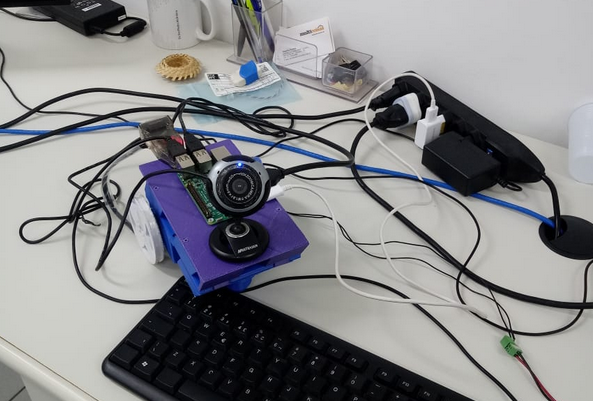
\includegraphics[scale=0.75, angle=0]{Figures/testefinal.png}
 	\caption{Exemplo de segmentação de cores}
 	\label{fig:testefinal}
 \end{figure}

\subsection{Tutoriais de Montagem do Robô}

\section{Kit Físico}

\subsection{Design}

\subsection{Fabricação}

\subsection{Montagem}
 



